\section{Real-World Driving Dataset and Reference Acquisition}
\label{sec:realworld}

Measuring gaze accuracy in real driving requires a trustworthy reference
for every fixation, under exactly the conditions in which gaze is to be
used. Unlike chessboard corners, road targets are not placed by the
experimenter and move through the image as car and head move. We built a
pipeline that makes such references practical and used it to measure
wearable gaze accuracy on the road.

\begin{figure}[t]
\centering
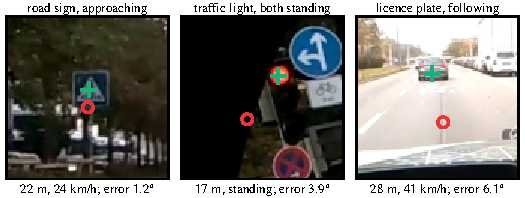
\includegraphics[width=\columnwidth]{figures/fig4_dataset.pdf}
\caption{Three real driving scenes with target class and relative motion
(top), LiDAR distance, GNSS speed and uncorrected median error (bottom).
Green cross: verified target centre; red circle: measured gaze.}
\label{fig:dataset}
\end{figure}

\subsection{Real-World Driving Dataset}

The evaluated benchmark contains 245 manually verified fixation scenes
(73{,}738 gaze samples) from 17 public-road drives of three participants,
two drivers and one front passenger, in sunny and cloudy daylight.
Driving-gaze datasets such as DR(eye)VE~\cite{palazzi2019dreyeve} and
BDD-A~\cite{xia2018bdda} provide gaze or attention maps for modelling
attention; our scenes instead pair each fixation with an independently
localised physical target and its context (Fig.~\ref{fig:dataset}). The
targets are licence plates (115), road signs (75) and traffic lights (55)
at 4.7--120\,m (median 27\,m, LiDAR-measured for 183 scenes), fixated
while approaching, passing, following, meeting oncoming traffic or
standing, with stationary and moving targets. Every scene also carries
vehicle speed or motion state, target side, road type and a scene
description.

\subsection{Efficient Reference Acquisition and Verification}

Participants announce the physical object they fixate, for example a
licence plate; the transcribed announcement defines the event and the
object class. Object detection proposes the target, and the measured gaze
only restricts the candidate-search region: the reference is the centre
of the detected object, not the gaze position. Point tracking, optical
flow and temporal consistency checks follow the target through the
fixation, and competing candidates or inconsistent tracks are flagged
automatically. In a dedicated Neon Player interface, every accepted
reference was manually verified, and a subset was additionally reviewed
by a second annotator; unidentifiable targets are excluded. As targets are small
and well defined (licence plates are typically about 6\,px or 0.4\dg{}
tall), their centres are precise relative to degree-scale gaze errors. Automation thus reduces manual
work to confirming or correcting proposals.

\subsection{Data Suitability and Real-World Accuracy}

Supporting checks qualify each sample for its downstream task: a
segmentation model trained on images from three vehicles separates the
windshield from windows, mirrors and the interior; native blink, eyelid
and saccade signals mark unusable intervals; and image-sharpness and
head-rotation checks, informed by experiments on exposure time, rotation
and marker detection, flag motion blur. References can be
collected in any drive, so accuracy can be re-checked repeatedly.

The verified references reveal a substantial accuracy problem. Without
person-specific correction, the median angular error on held-out scenes
is 3.96\dg{}, 1.48\dg{} and 6.00\dg{} for the three participants. Most of
it is systematic: the median signed offset makes up 91--99\% of each
participant's median scene error, mainly as a vertical shift of up to
6\dg{}, while target-relative dispersion stays at 0.5--1.7\dg{}. The same
references can correct this error; Section~\ref{sec:transfer} shows
reductions, for example, from 3.96\dg{} to 0.76\dg{} and from 6.00\dg{}
to 1.41\dg{}. The pipeline thus provides the evidence to discover,
characterise and correct gaze errors in the application environment. We
next examine which factors influence these wearer-dependent errors under
controlled conditions (Sec.~\ref{sec:controlled}) before evaluating
corrections on the road.
